% ============================================================
%  How Cheap Can Video Retrieval Be?
%  Build:  pdflatex main ; bibtex main ; pdflatex main ; pdflatex main
%  Local TeX Live lives in D:\video-retrieval\.texlive
% ============================================================
\documentclass[journal]{IEEEtran}
\usepackage{cite}
\usepackage{graphicx}
\usepackage{booktabs}
\usepackage{amsmath}
\usepackage{url}
\usepackage{tikz}
\usetikzlibrary{positioning,arrows.meta}
\usepackage[hidelinks]{hyperref}

\begin{document}

\title{How Cheap Can Video Retrieval Be?\\A Zero-Shot, CPU-Only Cost--Accuracy Study}

\author{\IEEEauthorblockN{Chengxuan Xie}\\[2pt]
\IEEEauthorblockA{Nanchang University\\
Nanchang, China\\
\texttt{chengxuan\_xie@email.ncu.edu.cn}}}

\maketitle

\begin{abstract}
Video retrieval systems are usually evaluated on accuracy and assumed to have a GPU
budget. We ask the complementary question: with zero training, zero annotation and a
single laptop CPU, how much accuracy is left, and where does the remaining cost go? We
build a text-to-video retriever from a frozen OpenCLIP ViT-B/32 encoder, one frame per
second, one 512-dimensional vector per frame, and exhaustive cosine search, and we
characterise its cost--accuracy curve on MSR-VTT test 1k. Recall@1 is 32.2\%, within 1.5\,pp of
the 30.7--31.2\% reported for zero-shot CLIP ViT-B/32 on this split \cite{ventura2024learning}, so
the pipeline is implemented correctly;
indexing the 1,000 clips takes 1{,}035.8\,s on four CPU threads. Varying the sampling rate
from 0.25 to 3.0\,fps --- the ceiling imposed by clips that are themselves stored at 3\,fps ---
changes indexing cost by 14$\times$ but Recall@1 by only 1.7\,pp, which a paired test cannot separate
from zero ($p=0.12$), which places the knee of the curve at 1\,fps and makes the sampling
rate the cheapest available knob. Per hour of video, the operating point costs
3.9--5.0 minutes of CPU time, 7.4\,MB of index and 0.0036\,kWh of electricity. A
component-level benchmark shows that decoding accounts for roughly a tenth of the
per-frame cost, so reducing the number of encoded frames, not the cost of video I/O, is
what matters. We also state the boundary of the design: beyond roughly $10^{7}$ frames a single
CPU can no longer answer a query in seconds, and either a GPU or an approximate index becomes
necessary.
\end{abstract}

\begin{IEEEkeywords}
video retrieval, contrastive vision-language models, zero-shot learning, cost modelling,
CPU inference
\end{IEEEkeywords}

% ------------------------------------------------------------
\section{Introduction}
% ------------------------------------------------------------

Video has become the largest source of unstructured data in most organisations, and
finding one specific moment in a large corpus is a routine need: the clip where a cyclist
crosses a junction, or the moment a chart appears on screen. Systems that answer such
queries well already exist. They also assume a well-provisioned pipeline: Craw indexes
large video collections on a machine with 128 CPU cores, 512\,GB of RAM and an RTX~4090
\cite{craw2026}, and LOVO encodes object-level representations at about 0.08\,s per
keyframe on an RTX~3090 \cite{lovo2025}. Because these figures are obtained on different
hardware from ours, we do not compare accuracies with such systems; instead we characterise
a different operating point, and Section~\ref{sec:related} explains why the two ends of the
design space are complementary rather than competing.

Under a zero budget, the binding constraint is not the choice of encoder but the number of
times the encoder is called. A conventional pipeline samples 30 frames per second, so one
hour of video costs 108{,}000 encoder calls. This paper asks what is left if that number is
divided by thirty and nothing else is changed.

Our contributions are threefold. First, a complete and reproducible retrieval system that
requires no training, no annotation and no GPU, together with the measurement scripts that
produce every number reported here. Second, a measured cost--accuracy curve on MSR-VTT:
across a 12$\times$ range of sampling rates --- up to every frame the corpus contains --- indexing
cost changes by 14$\times$ while Recall@1 moves by 1.7\,pp, which a paired test cannot separate from
zero ($p=0.12$), so the knee of the curve sits at 1\,fps. Third, an account of where the cost actually sits --- a component-level benchmark
that separates decoding from encoder computation --- and of the scale at which the design
should stop being used on a CPU.

We report zero-shot results: the system is never trained on the target videos, and its Recall@1
on MSR-VTT (32.2\%) is 32 points above the 0.1\% chance level. Four independent quantities --- frame
count per clip, implied count of correct retrievals, index size and random baseline --- agree with
each other and with the raw predictions (Section~\ref{sec:exp}), which we take as the evidence
that the pipeline is correct: a preprocessing or alignment error would drive the figure towards
chance. These figures agree with the 30.7--31.2\% reported for zero-shot CLIP ViT-B/32 baselines on
the same split \cite{ventura2024learning}, within one standard error, although the protocols differ
in frame count and pooling. The
result is below supervised state-of-the-art; the trade is deliberate.

% ------------------------------------------------------------
\section{Related Work}\label{sec:related}
% ------------------------------------------------------------

\noindent\textbf{Craw: multi-level queries over large video corpora.}
Craw unifies existence, dynamic and similarity queries over large-scale video datasets by
representing video as Video Semantic Units (trajectories, inter-object interactions and
temporal relations) and indexing them with a three-layer hybrid index that combines a
keyword inverted index with a tiered cluster index \cite{craw2026}. It reports up to two orders of magnitude
lower query latency than prior systems. However, it explicitly avoids frame skipping in order
to preserve tracking accuracy, which makes index construction heavy, and its reliance on a
closed-set detector limits queries to predefined object categories. Notably, Craw's two key
mechanisms --- semantic-preserving segmentation and trajectory simplification --- pursue the
same goal as our frame sampling: reducing the computation required per unit of video, albeit
at a finer granularity. Our approach can therefore be read as the cheapest point on the same
trade-off curve.

\noindent\textbf{LOVO: object-level queries.}
LOVO targets complex object queries, that is, retrieving segments that contain a specific
object configuration such as a red car running side by side with another car \cite{lovo2025}. To support
object-level localisation it partitions every keyframe into $K$ patches (roughly 2{,}040
patches for a 1080p frame with $32\times32$ patches), encodes each patch independently into a
768-dimensional vector, and predicts a bounding box and an open-vocabulary class embedding per
patch. Vectors are compressed with product quantisation and indexed with an inverted file, and
queries follow a coarse-recall then cross-modal rerank pipeline. This yields object-level
precision but multiplies the number of vectors per frame by $K$; the index reaches the order of
10\,GB for 30 million entities. The offline cost is justified by the observation that users are
not affected at query time; from a total-cost perspective, however, that offline work remains a
real expense.

\noindent\textbf{Bobsled: event patterns in streams.}
Bobsled addresses complex event processing over video streams, matching temporal patterns such
as a rolling stop followed by a right turn \cite{bobsled2025}. Rather than running an expensive recognition model
on every clip, it first applies a lightweight proxy model to obtain a per-clip event
distribution, then uses non-homogeneous Markov chains to estimate the probability that a window
matches the query pattern and prunes hopeless windows, and finally decides which remaining clips
are worth materialising with the expensive oracle model. It improves throughput by
2.4$\times$--11.6$\times$ over the state of the art without noticeable accuracy loss.
Bobsled is orthogonal to our work: it optimises throughput for streaming detection, whereas we
target offline, open-vocabulary content retrieval. Both, however, share the same underlying
strategy: avoid invoking the expensive model whenever a cheap signal can rule a candidate out.

\noindent\textbf{Positioning.}
Overall, prior systems optimise the upper bound of query expressiveness under the assumption of
a well-provisioned analytics pipeline. This work explores the opposite end of the design space:
what can be achieved with zero training budget, zero annotation and commodity CPU hardware. Our
contribution is therefore complementary rather than competitive: we quantify how much accuracy
must be sacrificed to obtain an order-of-magnitude reduction in construction cost.

% ------------------------------------------------------------
\section{System Design}
% ------------------------------------------------------------

\subsection{Overview}
The system has three stages and no learned component beyond the frozen encoder
(Fig.~\ref{fig:pipeline}). Offline, each
clip is decoded at one frame per second and every sampled frame is passed through OpenCLIP
ViT-B/32 \cite{cherti2023reproducible}, giving a 512-dimensional embedding that is
L2-normalised and stored as one row of a float32 matrix, 2{,}048 bytes per frame. Online, a
natural-language query is encoded by the text tower of the same model, scored against every
frame by a dot product, reduced to one score per clip by taking the maximum over its frames,
and the clips are then ranked. There is no index structure, no keyframe detection, no shot
segmentation and no temporal model: the index is a single matrix and retrieval is one linear
scan. The only parameter that changes the cost is the sampling rate, and every run writes its
configuration to a JSON file, so an index can always be traced back to the settings that
produced it.

\begin{figure}[t]
\centering
\resizebox{\columnwidth}{!}{%
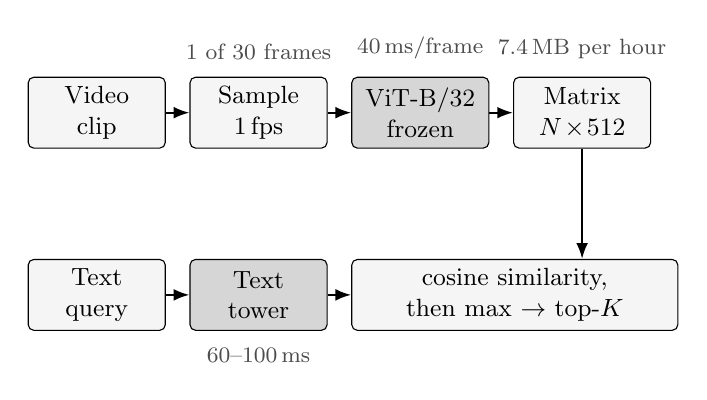
\begin{tikzpicture}[
  font=\small,
  box/.style={draw, rounded corners=2pt, align=center, minimum height=9mm,
              inner sep=2pt, text width=16mm, fill=black!4},
  net/.style={box, fill=black!16},
  arr/.style={-{Latex[length=2mm,width=1.5mm]}, thick},
  lab/.style={font=\footnotesize, text=black!70, align=center}
]
% ---- offline: indexing ----
\node (v) [box] {Video\\clip};
\node (s) [box, right=3mm of v] {Sample\\1\,fps};
\node (e) [net, right=3mm of s] {ViT-B/32\\frozen};
\node (m) [box, right=3mm of e] {Matrix\\$N\!\times\!512$};
\node [lab, above=1mm of s] {1 of 30 frames};
\node [lab, above=1mm of e] {40\,ms/frame};
\node [lab, above=1mm of m] {7.4\,MB per hour};
\draw [arr] (v) -- (s);
\draw [arr] (s) -- (e);
\draw [arr] (e) -- (m);
% ---- online: one query ----
\node (q) [box, below=14mm of v] {Text\\query};
\node (t) [net, right=3mm of q] {Text\\tower};
\node (c) [box, right=3mm of t, text width=40mm]
      {cosine similarity,\\ then max $\rightarrow$ top-$K$};
\node [lab, below=1mm of t] {60--100\,ms};
\draw [arr] (q) -- (t);
\draw [arr] (t) -- (c);
\draw [arr] (m.south) -- (m.south |- c.north);
\end{tikzpicture}}
\caption{The pipeline. Only the two shaded boxes run a neural network, and both are used
frozen: no training and no fine-tuning. Offline, each clip is decoded at 1\,fps and every
sampled frame becomes a 512-dimensional unit vector, so the index is a single $N\times512$
matrix. Online, a query costs one text embedding, one matrix--vector product and a max over
the frames of each clip. Labels give measured per-unit costs (Section~\ref{sec:cost}).}
\label{fig:pipeline}
\end{figure}

\subsection{Three Decisions and Their Costs}
Three decisions account for most of the cost and most of the accuracy. First, the encoder is
used zero-shot, which removes training entirely but leaves us below models tuned on the target
dataset; our Recall@1 of 32.2\% is within 1.5\,pp of the 30.7--31.2\% that zero-shot CLIP ViT-B/32
pipelines report on the same split \cite{ventura2024learning}, which suggests that the remaining
error comes from the encoder rather than from the pipeline.
Second, we sample at 1\,fps, discarding 29 of every 30 frames; brief events can therefore be
missed, although the ablation in Section~\ref{sec:fps} shows no significant loss at Recall@1 down
to 0.25\,fps, where Recall@10 falls by 2.4\,pp before correction for multiplicity. Third, one vector is stored per frame rather than per object, which removes
localisation but cuts the number of encoder calls per frame from $K$ to one; LOVO, which keeps
object-level vectors, pays on the order of $10^{3}$ times more per frame for that ability
\cite{lovo2025}.

\subsection{What We Deliberately Left Out}
We also chose not to build several components that the comparison systems require. Craw runs a
detector on every frame and never skips, because its queries are closed-set and structural;
LOVO adds a re-ranking stage over object proposals. Both are evaluated on fixed-camera
surveillance footage, whereas we target open-vocabulary retrieval over general web video. What
the three systems share is one principle: call the expensive model on as few units as possible.
Craw does this with an inverted index and three filtering layers, LOVO with a coarse-to-fine
recall stage, and this work by lowering the sampling rate itself, from 30 calls per second to
one and from $K$ units per frame to one. Two components are deliberately left out: product
quantisation, which changes the storage term rather than the compute term that dominates here, and
a two-stage retrieve-then-rerank scheme, which we take up in Section~\ref{sec:discussion}.

% ------------------------------------------------------------
\section{Cost Model}\label{sec:cost}
% ------------------------------------------------------------

\subsection{Five Cost Terms}
The total cost decomposes into five terms: fixed capital (hardware), compute (encoding), storage
(index), human (annotation and training) and access (the cheapest hardware able to run the system).
We set fixed and access cost to zero because the machine was already owned and the system needs only
a commodity laptop; this is an assumption about the deployment context, not a claim that no
hardware is required. Human cost is zero because the encoder is used zero-shot. The two remaining
design choices, sampling rate and aggregation, were fixed once by the ablation in
Section~\ref{sec:exp}, a one-off model selection rather than a per-query optimisation. What remains
to be measured is therefore the compute and storage cost of indexing, which the next subsection
quantifies.

\subsection{Cost of Indexing}
Indexing compute cost is $C_{\text{compute}} = N_{\text{frames}} \cdot t_{\text{frame}} \cdot
p_c$, where $N_{\text{frames}} = \sum_v (D_v \cdot r)$ is the number of sampled frames for
clips of duration $D_v$ at sampling rate $r$, $t_{\text{frame}}$ is the per-frame encoding time
and $p_c$ is the price of compute. Storage cost is $C_{\text{storage}} = N_{\text{frames}} \cdot
d \cdot b \cdot p_s$, with $d=512$ dimensions and $b=4$ bytes per component (float32). Only two
quantities require measurement, $t_{\text{frame}}$ and $N_{\text{frames}}$, and
$N_{\text{frames}}$ follows directly from the sampling rate; the two prices are assumptions
rather than measurements. Indexing, not querying, dominates the total cost: a query costs one
text encoding (60--100\,ms) plus an exhaustive dot product (1--6\,ms over
$2.5\times10^{3}$ frames), that is 0.06--0.11\,s, whereas indexing the same 1{,}000 clips takes
1{,}035.8\,s. The ratio is close to four orders of magnitude. Effort to reduce cost should
therefore be directed at indexing rather than at query latency.

\subsection{Measurement}
All timings were measured on the same 4-core laptop CPU described in Section~\ref{sec:exp}.
UCF-101 (2{,}462 frames at 1\,fps) was indexed three times, giving 197.6, 207.1 and 251.1\,s, a
median of 84\,ms per frame and a 27\% spread (max/min $-$ 1). MSR-VTT (16{,}036 frames) was indexed once, at
1{,}035.8\,s or 65\,ms per frame; its cost figures are therefore single-run estimates, and we
adopt the 27\% spread of the UCF repeats as the noise floor for both.

To locate the cost inside the pipeline, we timed the two stages separately on 20 clips of each
dataset, reusing the same sampling, preprocessing and batching code. Video decoding (seek,
decode, colour conversion) costs 5.6\,ms per frame on MSR-VTT and 6.7\,ms on UCF-101;
preprocessing plus the ViT-B/32 forward pass costs 40.4\,ms and 43.5\,ms respectively. The
encoder call is therefore roughly seven times more expensive than decoding. Summing the two stages
accounts for 77--84\% of an end-to-end run; the remainder is per-clip overhead that we did not
attribute, and the gap lies within the 27\% spread. The micro-benchmark runs are 15--22\% faster
than the full indexing runs above, which is also within that spread. Because the encoder term
dominates, the number of encoded frames rather than the speed of video I/O is the quantity to
reduce, which is what motivates the frame-level design.

\subsection{Normalised Cost per Hour of Video}
Normalised to one hour of video at 1\,fps, indexing costs 3{,}600 frames, 3.9--5.0 minutes of
CPU time, a 7.4\,MB index and 0.08\,h of machine time. At an assumed 45\,W system draw (a rough
estimate for the whole laptop, not measured with a power meter) that is 0.0036\,kWh, or about
0.03 US cents (0.2 CNY cents) at 0.55\,CNY/kWh. This figure covers electricity only; the
7.4\,MB index is priced separately and is not included. Processing at 30\,fps would require
108{,}000 frames, 2.0--2.5 hours and 221\,MB per hour of video, roughly 30$\times$ more on both
axes, and these 30\,fps entries are projections from the frame count rather than measurements.
What we did measure is that raising the sampling rate up to 3\,fps --- every frame the stored
clips contain --- produced no gain exceeding
one standard error; 30\,fps was not run. Table~\ref{tab:perhour} collects the three operating
points.

\begin{table}[t]
\centering
\caption{Cost per hour of video for three sampling rates. The 30\,fps row is projected from the
frame count; the other two are measured.}
\label{tab:perhour}
\begin{tabular*}{\columnwidth}{@{\extracolsep{\fill}}lccc@{}}
\toprule
Configuration & Frames & Indexing time & Index size \\
\midrule
30\,fps (projected)      & 108{,}000 & 2.0--2.5\,h  & 221\,MB \\
1\,fps (this work)       & 3{,}600   & 3.9--5.0\,min & 7.4\,MB \\
0.25\,fps                & 900       & 1.0--1.3\,min & 1.8\,MB \\
\bottomrule
\end{tabular*}
\end{table}

\subsection{Boundary of Validity}\label{sec:boundary}
The model also delimits its own validity. Valuing machine time at 50\,CNY/h --- the high
(GPU-rental) anchor of Section~\ref{sec:discussion} --- and assuming a
50$\times$ GPU speed-up, a 13{,}000\,CNY GPU repays itself at $N^{*}$ frames, where the
per-frame saving is the measured 65--84\,ms. This places the crossover between
$1.14\times10^{7}$ and $1.48\times10^{7}$ frames, that is 3{,}200--4{,}100 hours of video at
1\,fps. Because the calculation is a projection, its dependence on the price should be stated: the
crossover scales inversely with the value of machine time, so at 1\,CNY/h it moves to
$5.7$--$7.3\times10^{8}$ frames (roughly $1.6$--$2.0\times10^{5}$ hours of video) and the purchase never
repays itself within a plausible corpus. The GPU is therefore justified only where machine hours
are genuinely expensive, which is the reading we intend. A second and independent limit comes from search latency: exhaustive cosine search costs
0.5--2.4\,$\mu$s per frame in our measurements (1.2--5.8\,ms over 2{,}462 frames), so
extrapolated to $10^{7}$ frames it would need 5--25\,s per query. The two limits are of the same
order, $10^{7}$ frames, which we take as the operating range of a CPU-only deployment. Beyond it
we would keep the same compute-frugal pipeline and run it on a GPU, rather than change the
pipeline.

% ------------------------------------------------------------
\section{Experiments}\label{sec:exp}
% ------------------------------------------------------------

\subsection{Setup}
All experiments run on a single laptop CPU (Intel i5-1155G7, 4 cores / 8 threads, 15.8\,GB RAM)
with no discrete GPU. The encoder is OpenCLIP ViT-B/32 \cite{cherti2023reproducible}
(\texttt{laion2b\_s34b\_b79k}, 151.3\,M parameters, 605\,MB in fp32); the text tower of the same
model encodes queries, following the CLIP recipe \cite{radford2021clip}. Retrieval is exhaustive
cosine similarity over L2-normalised frame embeddings, implemented in NumPy. Timings use four
threads, matching the physical core count. Table~\ref{tab:setup} summarises the configuration.

\begin{table}[t]
\centering
\caption{System configuration.}
\label{tab:setup}
\begin{tabular}{@{}ll@{}}
\toprule
Item & Value \\
\midrule
CPU        & Intel i5-1155G7, 4 cores / 8 threads, 2.50\,GHz \\
Memory     & 15.8\,GB \\
GPU        & none \\
Framework  & PyTorch 2.15.0+cpu, 4 threads \\
Encoder    & OpenCLIP ViT-B/32, \texttt{laion2b\_s34b\_b79k} \\
Parameters & 151.3\,M (605\,MB fp32) \\
Training   & none (zero-shot) \\
Retrieval  & NumPy exhaustive dot product \\
\bottomrule
\end{tabular}
\end{table}

We evaluate on two datasets. MSR-VTT test 1k \cite{xu2016msrvtt} provides 1{,}000 clips of
15.7\,s on average, each paired with one human-written caption that we use as the query; every
query therefore has exactly one correct answer, so random Recall@1 is 0.1\%. UCF-101
\cite{soomro2012ucf101} is used only as a pipeline check: 405 clips from 10 action classes,
queried by class name, with roughly 40 correct clips per query and a random Recall@10 that
already reaches 65.5\%. No clip is used for training, because nothing is trained. Recall@K is
the fraction of queries whose correct clip appears in the top $K$ of the 1{,}000 (MSR-VTT) or
405 (UCF-101) candidates, and all queries are run against the full corpus rather than a reduced
candidate set.

\subsection{Main Results}
Indexing the 1{,}000 MSR-VTT test clips at 1\,fps yields 16{,}036 frame embeddings in
1{,}035.8\,s (65\,ms per frame) and a 32.84\,MB index. Retrieval reaches Recall@1 of 32.2\%,
Recall@5 of 55.6\% and Recall@10 of 66.5\%, against random baselines of 0.1\%, 0.5\% and 1.0\%
respectively (Table~\ref{tab:main}). A single query costs 60--100\,ms for text encoding and
1--6\,ms for the similarity search, so online cost is close to four orders of magnitude below
indexing cost.

\begin{table}[t]
\centering
\caption{MSR-VTT test 1k, 1\,fps, max aggregation. Random baseline is $K/N$ with $N=1{,}000$
clips and one correct answer per query.}
\label{tab:main}
\begin{tabular*}{\columnwidth}{@{\extracolsep{\fill}}lccc@{}}
\toprule
Metric & This work & Random & Gap \\
\midrule
Recall@1  & 32.2\% & 0.1\% & 32.1\,pp \\
Recall@5  & 55.6\% & 0.5\% & 55.1\,pp \\
Recall@10 & 66.5\% & 1.0\% & 65.5\,pp \\
\bottomrule
\end{tabular*}
\end{table}

Four independent checks support the implementation. The frame count per clip is 16.0, matching
15.7\,s at 1\,fps after per-clip rounding; an incorrect 30\,fps sampling would give about 471. The
number of
correct retrievals implied by the summary metric is 322, which matches the count in the raw
predictions. The index size is 16{,}036\,$\times$\,512\,$\times$\,4\,B\,=\,32.84\,MB. And the
random baselines equal $K/N$ exactly. These quantities are computed by different code paths yet
agree, which is the strongest available evidence that the pipeline is correct.

\subsection{Effect of the Sampling Rate}\label{sec:fps}
A natural design question is whether the frame-sampling rate affects retrieval quality. Since
action semantics are inherently temporal, we hypothesised that reducing the sampling rate from
1.0 to 0.25\,fps would noticeably degrade Recall. Contrary to this expectation, Recall@1 changed
only from 32.2\% to 30.7\%, while indexing cost fell by 3.7$\times$ (1{,}035.8\,s $\rightarrow$
277.5\,s) and the index shrank from 32.84\,MB to 8.90\,MB (Table~\ref{tab:fps},
Fig.~\ref{fig:cost}). A paired test gives $p=0.16$ for Recall@1 between 1.0 and 0.25\,fps, and
across the ten pairs that the five rates define nothing survives correction at either metric
(smallest corrected $p=0.17$); the largest uncorrected change is 2.4\,pp of Recall@10
(0.25 against 1.0\,fps), and it does not reappear against 3.0\,fps. We therefore read the sweep
as flat at both metrics, which makes the sampling rate the cheapest knob to turn. We sweep five
rates, 0.25, 0.5, 1.0, 1.5 and
3.0\,fps, the last being the ceiling of this axis: the stored clips are themselves 3\,fps, so
3.0\,fps indexes every frame except those of the twelve clips longer than 30\,s, cut at 90 frames
(24 frames, 0.05\%). From 1.0 to 1.5\,fps the cost grows 1.7$\times$ (1{,}759.8\,s) and the index
40\% (45.90\,MB); to 3.0\,fps it grows 3.8$\times$ (3{,}927.1\,s, 47{,}121 frames, 96.50\,MB) while
Recall@1 moves 32.2\%$\rightarrow$32.4\% and Recall@10 66.5\%$\rightarrow$65.2\%, neither
significant ($p=0.88$, $p=0.11$). The frame count grows 2.9$\times$ rather than 3$\times$ because
1\,fps keeps $\lceil N/3\rceil$ frames per clip. We therefore select 1\,fps as the operating point:
the lowest rate at which recall has reached its maximum within one standard error. A tighter budget
can use 0.25\,fps, which is 3.7$\times$ cheaper and 1.5\,pp worse at Recall@1; it is also the rate
that loses most at Recall@10 (2.4\,pp), before any correction for multiplicity. Section~\ref{sec:discussion}
repeats this ablation per query type and finds the same picture: the loss is not concentrated in
action-heavy queries, which would be the obvious place to look for one.

\begin{table}[t]
\centering
\caption{Sampling-rate ablation on MSR-VTT ($n=1{,}000$ queries). No pairwise difference survives
correction (smallest corrected $p=0.17$); the largest uncorrected change is 2.4\,pp of Recall@10
(0.25 against 1.0\,fps).
Clips are stored at 3\,fps, so 3.0\,fps is the ceiling: it indexes every frame except those of the
twelve clips past 30\,s, cut at 90 frames (0.05\% of the index).}
\label{tab:fps}
\begin{tabular*}{\columnwidth}{@{\extracolsep{\fill}}lcccccc@{}}
\toprule
fps & Frames & Build (s) & Index (MB) & R@1 & R@5 & R@10 \\
\midrule
3.0  & 47{,}121 & 3{,}927.1 & 96.50 & 32.4 & 56.1 & 65.2 \\
1.5  & 22{,}412 & 1{,}759.8 & 45.90 & 32.2 & 56.9 & 66.8 \\
1.0  & 16{,}036 & 1{,}035.8 & 32.84 & 32.2 & 55.6 & 66.5 \\
0.5  &  8{,}285 &   544.1 & 16.97 & 31.0 & 56.4 & 65.3 \\
0.25 &  4{,}344 &   277.5 &  8.90 & 30.7 & 55.0 & 64.1 \\
\bottomrule
\end{tabular*}
\end{table}

\begin{figure}[t]
\centering
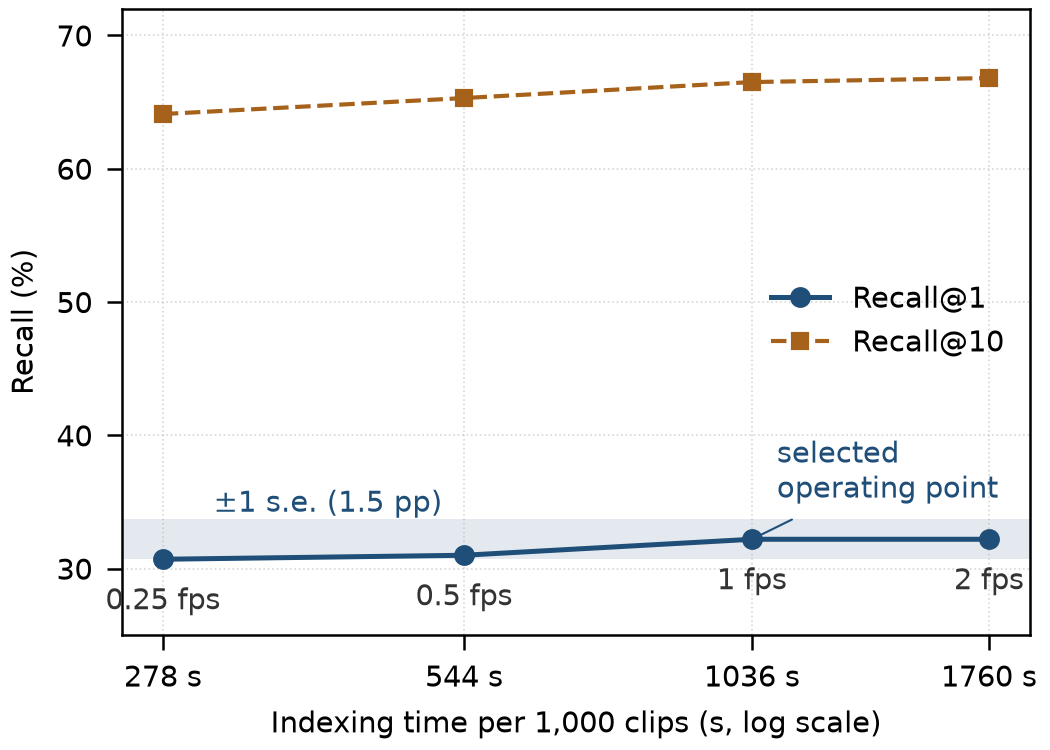
\includegraphics[width=\columnwidth]{fig_cost_accuracy.png}
\caption{Accuracy versus indexing cost on MSR-VTT test 1k (zero-shot CLIP ViT-B/32, exhaustive
search). Each point is a sampling rate; the horizontal axis is the measured indexing time for the
same 1{,}000 clips (log scale). A 12$\times$ range of rates changes cost by 14$\times$ but
Recall@1 by only 1.7\,pp, which a paired test between the endpoints cannot distinguish ($p=0.12$,
shaded band), so
higher rates buy no measurable accuracy and the knee sits at 1\,fps.}
\label{fig:cost}
\end{figure}

\subsection{Effect of Temporal Aggregation}
The choice between max- and mean-pooling of frame scores has no measurable effect on MSR-VTT
(differences $\leq$0.7\,pp, well within one standard error). We attribute this to the short,
single-shot nature of the clips: within a 15-second clip the visual content is largely
consistent, so the maximum and the mean frame score are strongly correlated. The same comparison
was inconclusive on the UCF-101 subset, where the metric is saturated. Temporal aggregation is
thus not an effective design variable at this granularity --- a conclusion that also explains why
LOVO abandons frame-level representations in favour of patch-level ones \cite{lovo2025}.

\subsection{Sanity Check on UCF-101}
On the UCF-101 subset, Recall@1, @5 and @10 are identical (90\%), indicating that the single
failing query cannot be recovered by increasing $K$. This confirms that the failure is semantic
rather than a matter of ranking depth. Because only 10 classes are present, roughly 10\% of the
corpus is relevant to any query and random Recall@10 already reaches 65.5\%; the metric therefore
carries little discriminative power. We use this dataset exclusively as a pipeline sanity check
and draw all quantitative conclusions from MSR-VTT.

\subsection{Timing and Statistical Conventions}
The timing protocol, its 27\% run-to-run spread and the split between video decoding and encoder
computation are reported in Section~\ref{sec:cost}. Every accuracy difference discussed below is therefore
compared against the 1.5\,pp standard error of Recall@1 at $n=1{,}000$: differences of 1.5\,pp or
less are treated as unresolved, and borderline cases are resolved by a paired McNemar test on the
same queries, with the raw $p$ reported alongside the value corrected for the number of tests in
the sweep.

% ------------------------------------------------------------
\section{Discussion}\label{sec:discussion}
% ------------------------------------------------------------

\subsection{Does Frame Rate Hurt Some Queries More Than Others?}
The flat curve of Fig.~\ref{fig:cost} averages over very different questions, and an average can
hide opposing effects. We therefore split the 1{,}000 queries into action (375), scene (64) and
object (561) queries with a keyword decision list, and recompute Recall@$K$ per class from the
same indexes --- the split costs no extra indexing --- at the four rates for which the labels were
evaluated (0.25, 0.5, 1.0 and 1.5\,fps). Table~\ref{tab:qtype} gives the result.
No class shows an effect at the 5\% level (all uncorrected $p>0.19$): the largest
change is the action class at 0.25\,fps, where Recall@1 falls from 37.3\% to 35.5\% (McNemar
$p=0.34$), well inside the 2.5\,pp standard error of a 375-query slice. What matters instead is the
question: at 1\,fps action queries reach 37.3\% against 28.7\% for object queries, a gap of
8.6\,pp ($z=2.8$, $p<0.01$), more than four times the largest sampling-rate change we actually
observe (1.8\,pp).
The cheap knob therefore removes cost without redistributing accuracy across query types, while
what the user asks moves recall by almost nine points. Because the labels are produced by rules rather than manual annotation, and the scene slice is
small ($n=64$), we treat the class-wise numbers as descriptive
(Section~\ref{sec:limits}).

\begin{table}[t]
\centering
\caption{Query-type stratification on MSR-VTT ($n=1{,}000$); labels come from a keyword decision
list, not manual annotation. Within a row, no sampling-rate difference reaches the 5\% level
(all uncorrected $p>0.19$). Between rows, action queries beat object queries by 8.6\,pp at 1\,fps.}
\label{tab:qtype}
\begin{tabular*}{\columnwidth}{@{\extracolsep{\fill}}l r cccc c@{}}
\toprule
 & & \multicolumn{4}{c}{Recall@1 (\%)} & Recall@10 \\
\cmidrule(lr){3-6}
Type & $n$ & 0.25 & 0.50 & 1.0 & 1.5 & 1.0\,fps \\
\midrule
action & 375 & 35.5 & 35.2 & 37.3 & 36.5 & 71.5 \\
scene  &  64 & 35.9 & 35.9 & 32.8 & 37.5 & 75.0 \\
object & 561 & 26.9 & 27.6 & 28.7 & 28.7 & 62.2 \\
\midrule
all    & 1000 & 30.7 & 31.0 & 32.2 & 32.2 & 66.5 \\
\bottomrule
\end{tabular*}
\end{table}

\subsection{Budget Allocation: What Extra Money Buys}
Because the curve of Fig.~\ref{fig:cost} is flat, a budget does not select a unique configuration; it
selects a set of configurations that are statistically indistinguishable. We therefore price the
increments directly. Moving from 0.25 to 0.5\,fps costs 267\,s of indexing per 1{,}000 clips and
returns 0.3\,pp; moving from 0.5 to 1\,fps costs 492\,s and returns 1.2\,pp; moving from 1 to
1.5\,fps costs 724\,s and returns 0.0\,pp; and the last step, to 3.0\,fps, costs a further
2{,}167\,s and returns 0.2\,pp. A point of Recall@1 thus costs between 410 and 890\,s of
laptop time in the cheapest part of the curve, while the top of the range pays 2{,}167\,s for
0.2\,pp, more than an order of magnitude worse. Any budget beyond roughly 1{,}040\,s per
1{,}000 clips is therefore better spent
elsewhere: the same
money applied to a second-stage re-ranker addresses the 34.3\,pp of headroom quantified in
Section~\ref{sec:scale} instead of 0.2\,pp, because a re-ranker scores ten candidates per query
rather than encoding the corpus again. This is the practical form of the trade-off: below 1\,fps
the budget buys at most about one point of Recall@1, which sits at the edge of the noise band;
above it the money is all but wasted.

\subsection{When Does Storage Overtake Compute?}
The common expectation is that storage eventually dominates the cost of a video index. For a
frame-level index it does not, at least not as the corpus grows. One encoded frame costs 65\,ms of
laptop time and occupies 2{,}048\,B. Writing $P$ for the price of machine time in CNY per hour,
compute is $1.8\times10^{-5}P$\,CNY per frame, while the same frame costs
$5.1\times10^{-5}$\,CNY of memory (25\,CNY/GB) or $1.0\times10^{-6}$\,CNY of solid-state storage
(0.5\,CNY/GB). Both terms are linear in the number of frames, so no corpus size makes one overtake
the other; the crossover is in the price. The two terms are equal at $P=2.8$\,CNY/h for a
memory-resident index and at $P=0.06$\,CNY/h for an SSD index. Priced as electricity only --- which
our own energy estimate in Section~\ref{sec:cost} puts at roughly 0.03\,CNY per machine hour --- storage
dominates a memory-resident index by two orders of magnitude; priced as rented GPU-class time, tens
of CNY per hour, compute dominates by one order of magnitude. Since our deployment assumes an
already-owned laptop, neither term is negligible, and the honest reading is that the ranking is a
statement about how machine time is priced rather than about the corpus. What does grow with $N$ is
capacity: 15.8\,GB holds $7.7\times10^{6}$ frames, about 2{,}140 hours of video at 1\,fps, and at
that size the index stops being resident in a commodity laptop.
Compression then becomes mandatory, which is why LOVO invests in product quantisation at
$3\times10^{7}$ entities while we can still afford float32 below the wall; the remedy here is the
same, and off-the-shelf vector libraries already provide it \cite{johnson2019faiss}.

\subsection{Scale Limit and Measured Headroom}\label{sec:scale}
Exhaustive search scales linearly: 1.2--5.8\,ms for $2.5\times10^{3}$ frames extrapolates to
5--25\,s for $10^{7}$ frames, the scale at which approximate indexes become mandatory. This
delineates the regime in which our design is viable and explains why LOVO, which targets tens of
millions of entities, devotes most of its engineering effort to index compression. In the other
direction, 34.3\,pp of our queries place the correct clip between ranks 2 and 10, so a perfect
re-ranker over the top-10 would lift Recall@1 to 66.5\%. This quantifies the headroom of the
coarse-to-fine architecture adopted by LOVO and motivates a cheap verification stage as future
work.

\subsection{Why Queries Fail}
Failure analysis reveals three distinct causes rather than a single deficiency. First,
genre-level captions such as ``cartoon show for kids'' are under-specified: many clips in the
corpus are cartoons, so no visual evidence can single out the intended one. Second, queries that
require reading on-screen content (``someone playing a game in a computer'') exceed what a
whole-frame embedding can capture. Third, long multi-clause captions dilute the text embedding,
so a query carrying three facts retrieves worse than a short query for any single one. Each cause
points to a different remedy --- query rewriting, patch-level or OCR representations, and
multi-vector queries --- which is why we do not attribute the failures to insufficient model
capacity.

% ------------------------------------------------------------
\section{Limitations}\label{sec:limits}
% ------------------------------------------------------------

Three limitations follow directly from the measurements. First, frame-level CLIP embeddings
discard motion: a query for ``basketball dunk'' retrieves only generic basketball clips, with
scores compressed into a 0.010 band. Second, the system cannot localise events precisely, since
1\,fps bounds temporal resolution to one second; timestamps are therefore accurate to about
$\pm$1\,s and no finer. Third, all results are zero-shot and single-stage; the 34.3\,pp gap
between Recall@1 and Recall@10 marks the accuracy that a second stage could recover. Beyond
these, the boundary derived in Section~\ref{sec:boundary} is a property of the method rather than a defect: at
roughly $10^{7}$ frames a query would take 5--25\,s, so either a GPU or an approximate index
becomes necessary.

% ------------------------------------------------------------
\section{Conclusion}
% ------------------------------------------------------------

We measured what a video retrieval system costs when the budget is a laptop. Freezing a CLIP
encoder, sampling one frame per second and searching exhaustively gives Recall@1 of 32.2\% on
MSR-VTT, at 3.9--5.0 minutes of CPU time and 7.4\,MB per hour of video. The most useful result is
negative: using every frame the stored clips contain instead of one per second, a 3$\times$
increase in sampled frames, costs nearly four times more and buys nothing measurable, so
the accuracy of this class of system is limited by the encoder rather than by the frame rate. A
component-level benchmark confirms that the encoder, not video I/O, is the dominant term, which
is why the sampling rate is the right knob to turn. Two extensions follow directly: a second-stage
re-ranker, with an upper bound of 34.3 points on our data, and compression for corpora beyond
$10^{7}$ frames, where CPU-only search ceases to be appropriate.

\bibliographystyle{IEEEtran}
\bibliography{refs}

\end{document}

